\section{Introduction}
The Special Supplemental Nutrition Program for Women, Infants, and Children
(WIC) provides nutritious foods and nutrition counseling for low-income pregnant or postpartum women, infants, and children under the age of five. To be eligible for WIC, one needs to live in households with family incomes under 185\% of federal poverty line or have participated in other welfare programs such as Medicaid, Temporary Assistance to Needy Families (TANF), or Special Supplemental Nutrition Program (SNAP).  WIC participation has been linked to improved birth and children outcomes \citep{hoynes2011can,kreider2016identifying,chorniy2020does}. However, total WIC participation has been declining by approximately 3 millions in last decade. In 2009, WIC served around half of all infants born in the U.S. This number dropped to 30\% in 2021 (as in Figure \ref{trend1}). Between 2002 and 2022, WIC transitioned from paper vouchers to electronic benefit transfer (EBT) cards. This payment reform was expected to encourage WIC participation by reducing transaction costs and welfare stigma associated with using paper vouchers. Empirical evidence, on the other hand, shows mixed findings. For example, \cite{hanks2019paper} find that WIC EBT increases WIC
redemption in Ohio. \cite{li2022impacts} find no significant impact of WIC EBT on the share of WIC enrollment in Oklahoma. Finally, \cite{meckel2020cure} finds WIC EBT decreases the number of WIC births in Texas. One common concern in previous work is that results are based on individual states thus difficult to generalize. In this paper, we evaluate the impact of WIC EBT implementation on WIC participation by linking the WIC EBT roll-out schedule across virtually all counties in the U.S. to Vital Statistics Natality Data, which began reporting WIC status of live births in 2009. Live births participated in WIC (henceforth, WIC births) can plausibly capture the change in total WIC participation because the ratio of WIC births to total WIC participants maintain 20\% from 2009 (as in Figure \ref{trend2}). The share decline mildly after pandemic, but we show that our results do not change after dropping data after 2019.

\begin{figure}
	\begin{subfigure}[t]{.5\textwidth}
		\centering
		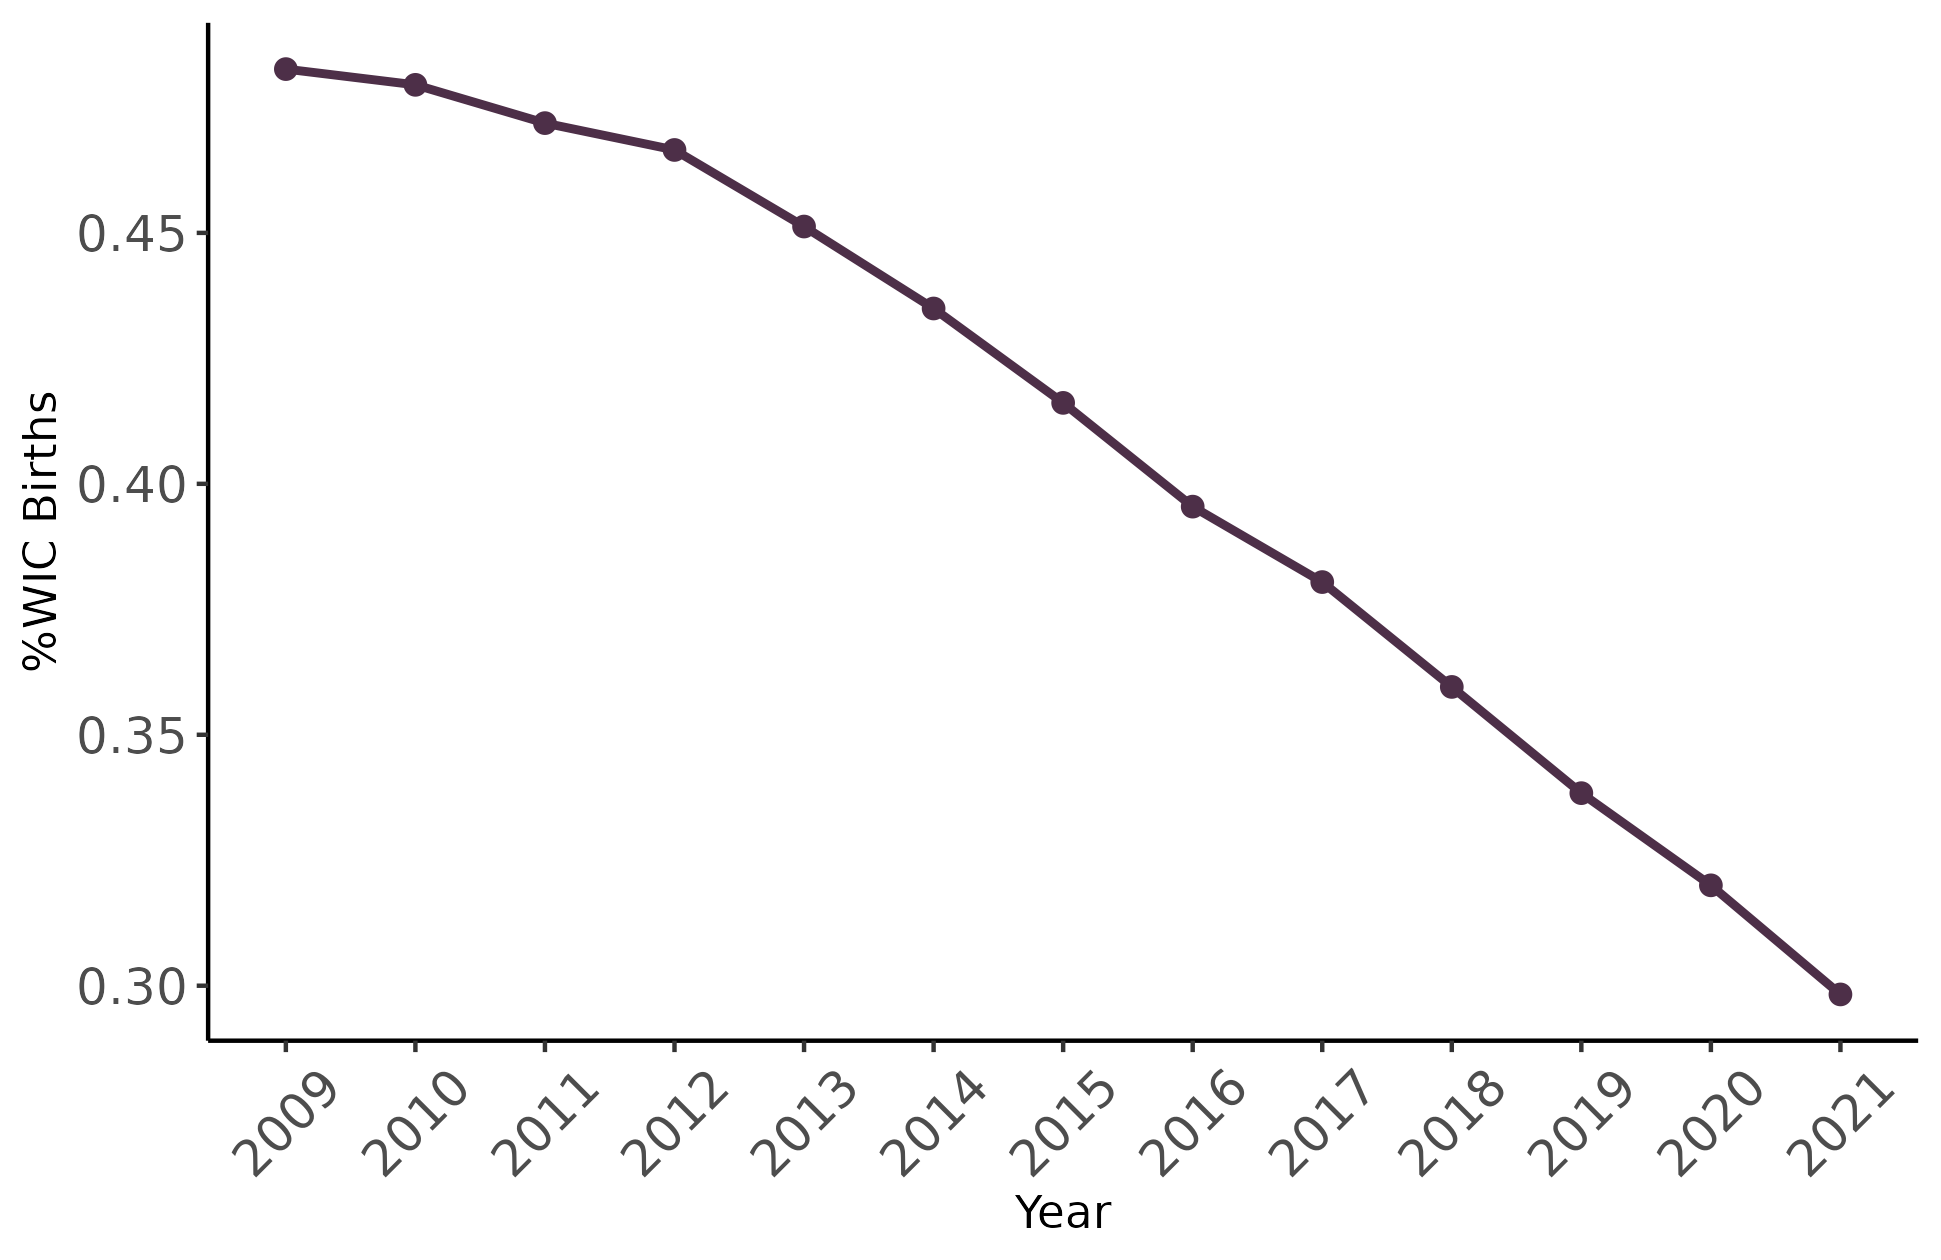
\includegraphics[width=\textwidth]{wic_par_sum_res.png}  
		\caption{\% Births Participated in WIC}
		\label{trend1}
	\end{subfigure}
	\begin{subfigure}[t]{.5\textwidth}
		\centering
		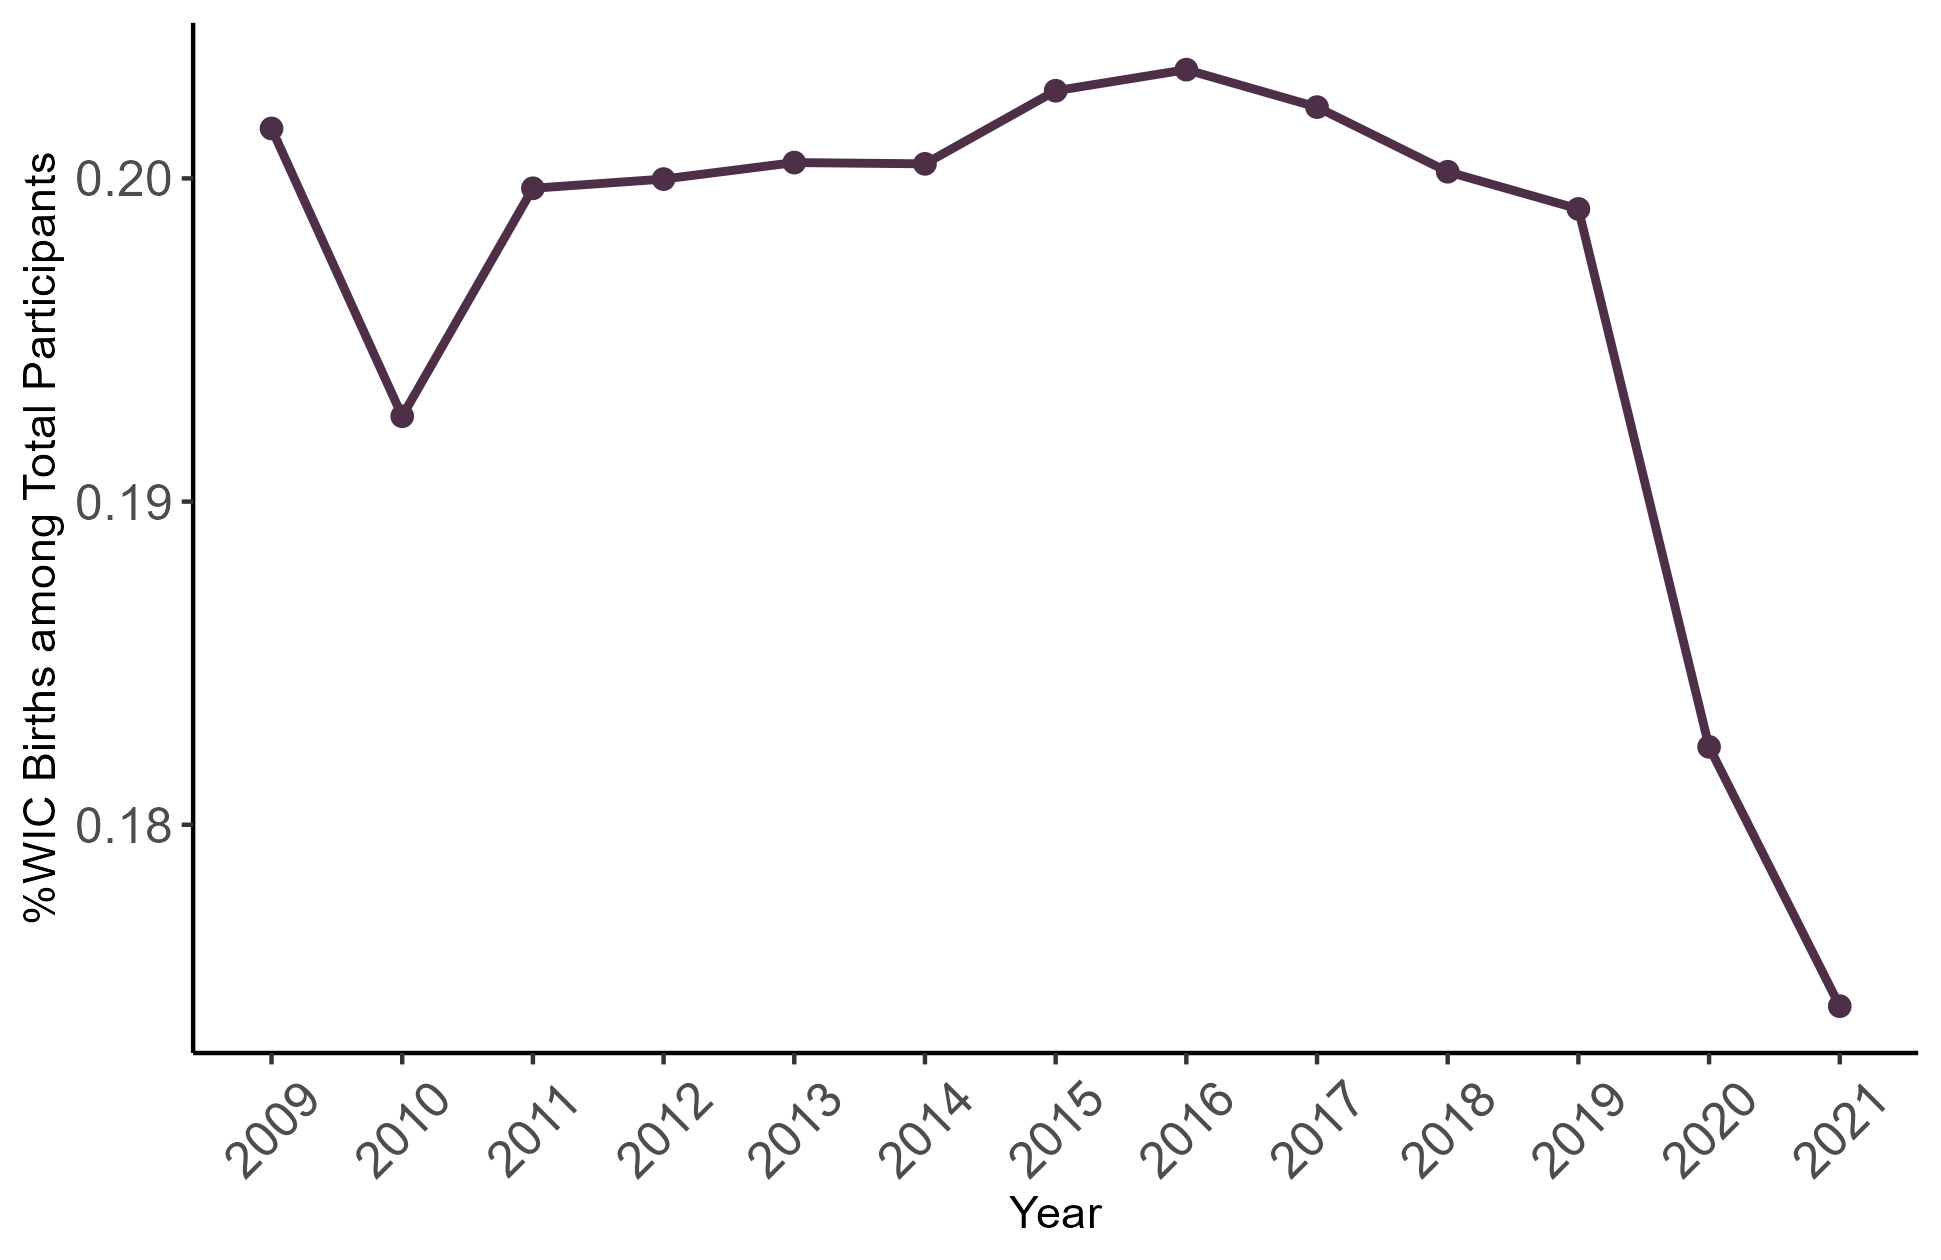
\includegraphics[width=\textwidth]{wic_par_pc.png}  
		\caption{The Ratio of WIC Births to All Participants}
		\label{trend2}
	\end{subfigure}
	\caption{\textsc{Trends of WIC Births}}
	\label{trend}
	\footnotesize
\end{figure} 

This paper builds on \cite{meckel2020cure}, which leverages WIC EBT rollout in Texas to study both vendors' and consumers' responses to EBT transition. She finds that EBT implementation causes vendors to drop out and reduces program take-up. We extend Meckle's analysis on program take-up to national level by collecting WIC EBT roll-out schedule across virtually all counties in the U.S. Our preferred estimates show results opposite to Meckle's findings in Texas: WIC EBT significantly increase WIC participation among mothers who are more likely eligible for WIC. Specifically, WIC participation increase by 9.18\% among less-educated and unmarried mothers after EBT implementation and by 14.82\% if the mothers are also minority. We find that Meckle's results on WIC take-up pick up the trend of numbers of live births and thus cannot tease out causal impact of EBT. Our preferred estimators using Meckle's data show that impact of EBT on WIC participation in Texas is in fact consistent with our main results based on much larger amounts of counties. Our results are robust to sample selection, estimation methods, timing of data collection, and definition of likely eligible sub-population.

We make several contributions to existing literature. First, we contribute to literature evaluating impacts of WIC EBT by collecting nationwide, county-level EBT rollout schedule and providing more credible empirical evidence based on much larger sample. Second, we add to literature on behavioral response to detail change in the design of food assistance programs. Finally, we contribute to literature discussing factors affect take-up of public program.